%!TEX root = ../NCVC6.tex

\mysection{手作業での修正とシミュレーション}

\vspace*{1zh}
 2つ目の小細工です.
出力されたファイルをメモ帳などのエディタで開き,順番に末尾へ追加します.
結合部分でM30を取り除いたりZ軸原点復帰を入れるなど,適宜変更してください.
今回のメインテーマであるワーク座標系設定の埋め込みも忘れずに.

\begin{lstlisting}[caption=編集後のNCプログラム,numbers=none,label=lst:gcode.txt]
%
G90G54G00X0Y0  → G92は削除
S3000M3
(Layer="CAM_54" start)
(R2.000 start)
G99G81X12.017Y10.925Z-20.R5.F60
(End of CircleData)
G80
G00Z10.
G91G28Z0  → M30は削除 安全のためZ軸機械原点復帰

G90G55G00X0Y0  → 次のワーク座標系の設定と移動
(Layer="CAM_55" start)
(R2.000 start)
G99G81X12.89Y-7.651Z-20.R5.F60
X13.108Y-15.509
(End of CircleData)
G80
G00Z10.
G91G28Z0
以下省略
\end{lstlisting}

\vspace*{1zh}
 次にNCVCの[工作機械の設定]でワーク座標系のオフセットを設定します.
今回はCADデータに合わせて図\ref{fig:work} のように設定しました.
実際には工作機械に登録されている座標に合わせると,より現実に近い動きになると思います.

\begin{figure}[H]
\centering
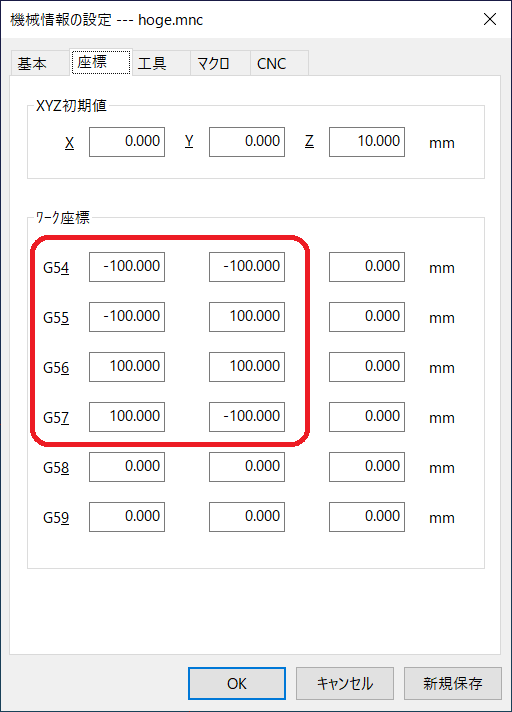
\includegraphics[scale=0.7]{No4/fig/work.png}
\caption{工作機械の設定(ワーク座標設定)}
\label{fig:work}
\end{figure}

 この状態で結合編集後のGコードをシミュレーションすると,図\ref{fig:simu1} のようになります.

\begin{figure}[H]
\centering
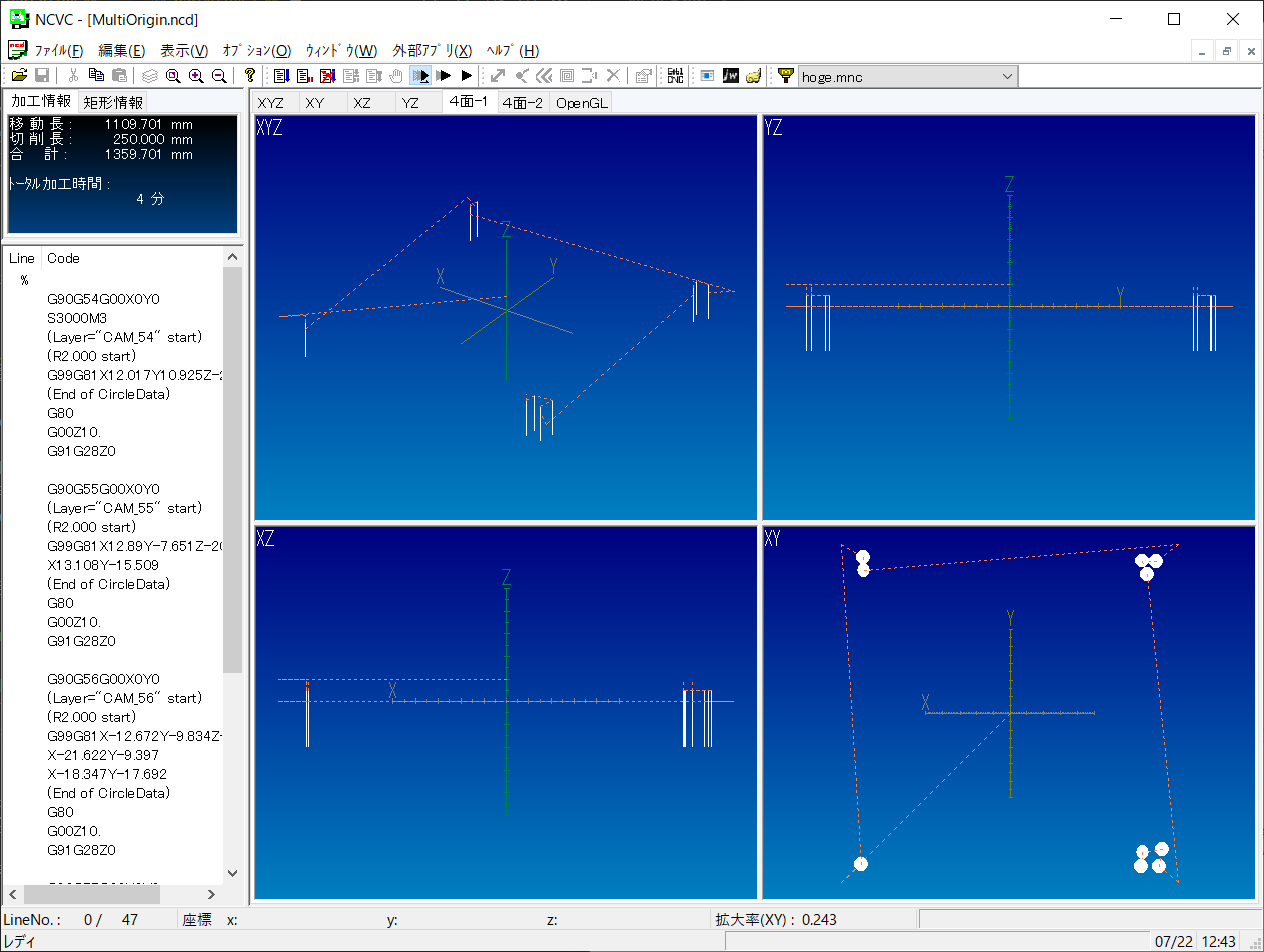
\includegraphics[scale=0.5]{No4/fig/simu1.png}
\caption{結合編集後のシミュレーション結果}
\label{fig:simu1}
\end{figure}

 NCVCのシミュレーションでG28リファレンス復帰はサポートされていないので,Z軸機械原点復帰は移動していないように見えますが,これは仕様です.
無理矢理感は否めませんが,この手順で複数の加工原点に対応した加工データの生成とそのシミュレーションができていると思います.

 他にも手はあると思いますので,いろいろ使いこなしてみてください.
